\section{Exponential tails}

\subsection{The model}\label{subsec:The_model}
Consider the BRW $(\widehat{\bb{T}}, \widehat{V})$ governed by the point process $\widehat{\scr{L}} \in \frak{M}$ with logarithmic moment generating function $\widehat{\psi}$. Assume that both of $\pm \widehat{\scr{L}}$ satisfy (\ref{eqn:BRW_generator_finite}), in other words 
\begin{equation}\label{ass:DacyingTails}
\exists\, \delta_- < 0 < \delta_+\, \text{ such that } \E \sum\limits_{|x| = 1} e^{\delta_- \widehat{V}(x)} < \infty\, \text{ and }\, \E \sum\limits_{|x| = 1} e^{\delta_+ \widehat{V}(x)} < \infty. 
\end{equation}
Further assume that $\widehat{\psi}$ satisfies (\ref{eqn:t*exists}). Let $(\widehat{X}_n)_{n \geq 0}$ be the corresponding $N$-BRW and write $\max \widehat{X}_n$ and $\min \widehat{X}_n$ for the position of the right- and leftmost particle of $\widehat{X}_n$. Our goal in this chapter will be to prove that $\hat{v}_N \defeq \lim_{n \to \infty} n^{-1}\max\widehat{X}_n$ exists almost surely and in $L^1$ and that it converges to $\hat{v} \defeq \lim_{N \to \infty} \hat{v}_N$ at rate $o((\log N)^{-2})$. \\

Apply the transformation (\ref{eqn:transformation}) to get the BRW $(\bb{T}, V)$ with point process $\scr{L}$ and logarithmic moment generating function $\psi$ that satisfies (\ref{eqn:BRW_V_Ass}) and observe that the associated random walk $(S_n)_{n \geq 0}$ with step distribution $X$ then satisfies (\ref{eqn:RWCentred}). Let $X \defeq (X_n)_{n \geq 0}$ denote the $N$-BRW with point process $\scr{L}$ and take $X_0 \in \frak{M}_N$ deterministic. Assuming it exists, $v_N \defeq \lim_{n \to \infty} n^{-1} \max X_n$ is related to $\hat{v}_N$ by 
\begin{equation}\label{eqn:speed_relation}
v_N + \widehat{\psi}(t^*)= \hat{v}_N t^*, 
\end{equation}
as can be seen from (\ref{eqn:transformation2}). We now record three lemmas that will be useful later in this section. 

\begin{lemma}\label{lem:ExpTailsMax}
Let $\tau \in L^1$ be an $\N$-valued random variable and let $(\epsilon_n)_{n \geq 1}$ be an i.i.d. sequence of random variables with exponentially decaying tails, independent of $\tau$. Then $M \defeq \max_{1 \leq n \leq \tau} \epsilon_n$ has exponentially decaying tails. 
\end{lemma}

\begin{proof}
Let $C, \gamma, t_0 > 0$ be such that $\Pr{|\epsilon_1| \leq t} \geq 1 - C e^{- \gamma t}$ for all $t > t_0$. Then for $t > t_0$ large enough, Bernoulli's inequality gives 
\begin{align*}
\Pr{M > t} &\leq 1 - \Ex{\Pr{|\epsilon_1| \leq t}^\tau} \leq 1 - \Ex{(1 - C e^{-\gamma t})^\tau} \\
		   &\leq 1 - \Ex{1 - C e^{- \gamma t} \tau} = \underbrace{C\, \Ex{\tau}}_{< \infty} e^{- \gamma t}. 
\intertext{Similarly, looking at the lower tail we get}
\Pr{M < -t} &\leq 1 - \Ex{\Pr{|\epsilon_1| \leq t}^\tau} \leq C\, \Ex{\tau} e^{- \gamma t}. 
\end{align*}
\end{proof}

\begin{lemma} \label{lem:ExpTailBound}
For all large enough $a$, 
\begin{equation}
x \Ind_{\{x \geq a\}} \leq e^{x - a/2}, \qquad\forall\, x \in \R. 
\end{equation}
\end{lemma}
\begin{proof}
Differentiate the map $f:x \mapsto \exp(x - a/2) - x$ to find that for large enough $a$, f is increasing on $[a, \infty)$. Noting that $f(a) \geq 0$ for all large $a$ concludes the proof.  
\end{proof}

\begin{lemma}\label{lem:ExpTailsGW}
Let $(M_n)_{n \geq 0}$ be a supercritical Galton-Watson process with offspring distribution $X$ and let $\mu \defeq \E X > 1$. If $M_0 = 1$ then for all $\mu > \phi > 0$ we have $0 < \liminf_n \Pr{M_n > \phi^n}$. 
\end{lemma}

\begin{proof}
By the monotone convergence theorem we can take $R$ large enough so that $\widetilde{\mu} \defeq \Ex{R \land X} > 1$. Let $(\widetilde{M}_n)_{n \geq 0}$ be the Galton-Watson process with offspring distribution $\widetilde{X} \defeq R \land X$ which by assumption is also supercritical. As $\widetilde{X}$ is bounded, Theorem 1 in Section 6, Chapter 1 of \cite{athreya2004branching} gives $\widetilde{\mu}^{-n} \widetilde{M}_n \to M$ almost surely for some $M \geq 0$ with $\Pr{M > 0} > 0$ by Theorem 2 of the same section. By the obvious coupling $\Pr{M_n > \phi^n} \geq \Pr{\widetilde{M}_n \mu^{-n} > \phi^n \mu^{-n}}$ so that $\liminf_{n \to \infty} \Pr{M_n > \phi^n} \geq \Pr{M > 0} > 0$. 
\end{proof}

\subsection{Properties of the model}
For all $t\in\R$ and $k \geq 1$ we have $0 \leq e^{t\, \scr{L}_{n,j}(k)} \leq \sum_{|x|=1} e^{t\, V(x)}$ so by (\ref{ass:DacyingTails}) the $\scr{L}_{n,j}(k)$ have finite moment generating function in a neighbourhood of zero which implies exponentially decaying tails. It follows that $\min X_n$ and $\max X_n$ are integrable and hence finite. Let $d(X_n) \defeq \max X_n - \min X_n$ be the diameter of $X_n$. We have the following result, analogous to Corollary 1 of \cite{exp_tails}: 

\begin{proposition}\label{prop:diameter}
For any $N \geq 1$ and initial population $X_0 \in \frak{M}_N$, we have 
\begin{equation*}
\frac{d(X_n)}{n} \xrightarrow[n \to \infty]{a.s.,\, L^1} 0. 
\end{equation*}
\end{proposition}

\begin{proof}
Let $u \in \N_+$ and for $n \geq u$ consider the process $X$ in the timeframe $\bbracket{n - u, n}$. Define $m \defeq \min\{ \scr{L}_{i, j}(N) \mid\, i \in \bbracket{n-u, n-1},\, j \in [N]\}$ and $M \defeq \max\{ \scr{L}_{i, j}(1) = \max\scr{L}_{i,j} \mid\, i \in \bbracket{n-u, n-1},\, j \in [N]\}$. By Lemma \ref{lem:ExpTailsMax} both $m$ and $M$ are integrable. Write $y \defeq \max X_{n - u}$ for the rightmost particle's position at time $n-u$. Suppose that for each $k \in [u]$ we have $\min X_{n - u + k} < y + k m$. As all steps during branching are $ \geq m$, this implies in particular that the descendants of the particle at space-time point $(y, n-u)$ survive all selection steps until time $n$. Consider a Galton-Watson process $G \defeq (G_n)_{n \geq 0}$ with offspring distribution $\scr{L}$ coupled with the descendants of $(y, n-u)$ and consider the event $A_u \defeq \{ G_u > N\}$. Since $\Ex{\#\scr{L}} > 1$ and $\#\scr{L} \geq 1$ almost surely, $\Pr{A_u} \to 1$ as $u \uparrow \infty$. Since at most $N$ descendants of $y$ can be alive at any time, $\min X_{n - u + k} \geq y + k_0 m$ for some $k_0$ almost surely on $A_u$. By the definition of $m$ this must also hold for all $k \in \bbracket{k_0, u}$, in particular for $k = u$. Noting that $\max X_n \leq y + u M$, it follows that 
\begin{equation}\label{eqn:ExpTailDiamUpperBound}
d(X_n)\Ind_{A_u} \leq u (M - m), 
\end{equation}
with probability one. Fix $\epsilon > 0$ and take $u$ large enough so that $\Pr{A_u^c} < \epsilon^2$. Consider the decomposition
\begin{equation}\label{eqn:ExpTailsDiamDecomp}
\frac{d(X_n)}{n} = \frac{d(X_n)}{n} \Ind_{A_u} + \frac{d(X_n)}{n} \Ind_{A_u^c}. 
\end{equation}
Taking expectations and then taking $n$ to infinity, the first term vanishes by (\ref{eqn:ExpTailDiamUpperBound}). The second term is upper bounded by $(\Pr{A_u^c} \Ex{d(X_n)^2 / n^2})^{1/2}$ using Hölder's inequality. A rough bound on $d(X_n)$ suffices: $d(X_n)$ is stochastically dominated by the sum of $n$ i.i.d. copies of $\max_{j \in [N]} \scr{L}_{0, j}(1) - \min_{j \in [N]} \scr{L}_{0,j}(N)$. Since the $\scr{L}_{n,j}(k)$ have exponentially decaying tails, by Lemma \ref{lem:ExpTailsMax} this yields $\Ex{d(X_n)^2} = \cal{O}(n^2)$ which implies that the second term in \ref{eqn:ExpTailsDiamDecomp} is $\cal{O}(\epsilon)$. Taking $\epsilon$ to zero concludes the proof of $L^1$ convergence. Almost sure convergence is a consequence of the proof of the next Proposition. 
\end{proof}

\begin{proposition}[{{\cite[Proposition 2]{exp_tails}}}]\label{prop:ExpTailsSpeedExistence}
There exists $v_N \in \R$ such that for any initial population $X_0 \in \frak{M}_N$ the following holds almost surely and in $L^1$:
\begin{equation}
\lim\limits_{n \to \infty} \frac{\min X_n}{n} = \lim\limits_{n \to \infty} \frac{\max X_n}{n} = v_N. 
\end{equation}
\end{proposition}

\begin{proof}
First we treat the case $X_0 = N \delta_0$. Recall the definition of $(\scr{L}_{n, j})_{n \geq 0, j \in [N]}$ from the construction of $X$. For each $l \geq 0$ we define the process $(X^l_n)_{n \geq 0}$ by shifting the origin of time by $l$. More precisely, given the process up to time $n \geq 0$, define $X^l_{n+1}$ to be given by the $N$ rightmost particles of 
\begin{equation}
\sum_{j = 1}^N \sum_{l \in \scr{L}_{n + l, j}} \delta_{X^l_n(j) + l}. 
\end{equation}
It is clear that each $(X^l_n)_{n \geq 0}$ has the same distribution as the $N$-branching random walk with offspring $\scr{L}$. Start $(X^l_n)_{n \geq 0}$ from $N \delta_0$ for each $l \geq 0$ so that $(X^0_n)_{n \geq 0} = (X_n)_{n \geq 0}$ almost surely. From Lemma \ref{lem:monotonicity} it follows easily that 
\begin{equation}\label{eqn:subadd}
\max X^0_{n + m} \leq \max X^0_n + \max X^n_m \qquad \forall\, n,m \geq 0. 
\end{equation}
For clarity define $Z_{i,j} = \max X^i_{j - i}$ for $0 \leq i \leq j$. Then (\ref{eqn:subadd}) reads $Z_{0, j} \leq Z_{0,i} + Z_{i,j}$ for all $0 \leq i \leq j$, which is familiar territory for Kingman's Subadditive Ergodic Theorem. We postpone showing that the conditions of the theorem hold to Lemma \ref{lem:ExpTailsKingmanHolds}. Applying the theorem yields $\lim_{n \to \infty} n^{-1} \max X_n = \lim_{n \to \infty} \Ex{n^{-1} \max X_n} = \inf_n \Ex{n^{-1} \max X_n} = v_N \in \R$ where the first limit is almost sure. Noting that the process $(-X_n)_{n \geq 0}$ also satisfies the necessary conditions thanks to (\ref{ass:DacyingTails}), we can deduce from the identity $\min X_n = - \max (-X_n)$ that $\lim_{n \to \infty} n^{-1} \min X_n = \lim_{n \to \infty} \Ex{n^{-1} \min X_n} = \inf_n \Ex{n^{-1} \min X_n} = \tilde{v}_N \in \R$ exists too, where the first limit is almost sure. From the proof of Proposition \ref{prop:diameter} we immediately get $\tilde{v}_N = v_N$ by uniqueness of $L^1$ limits, which gives $\lim_{n\to\infty} n^{-1}d(X_n) = v_N - \tilde{v}_N = 0$ almost surely as claimed. The proof is complete in the case $X_0 = N \delta_0$. By translation invariance of the dynamics of the system the result also follows for initial conditions of the form $N \delta_{x_0}$ for any $x_0 \in \R$. Finally, for arbitrary $X_0 \in \frak{M}_N$ note that the result is a consequence of Lemma \ref{lem:monotonicity} and a sandwiching argument between the initial configurations $N \delta_{\min X_0}$ and $N \delta_{\max X_0}$. 
\end{proof}

\begin{wrapfigure}{R}{0.5\textwidth}
\centering
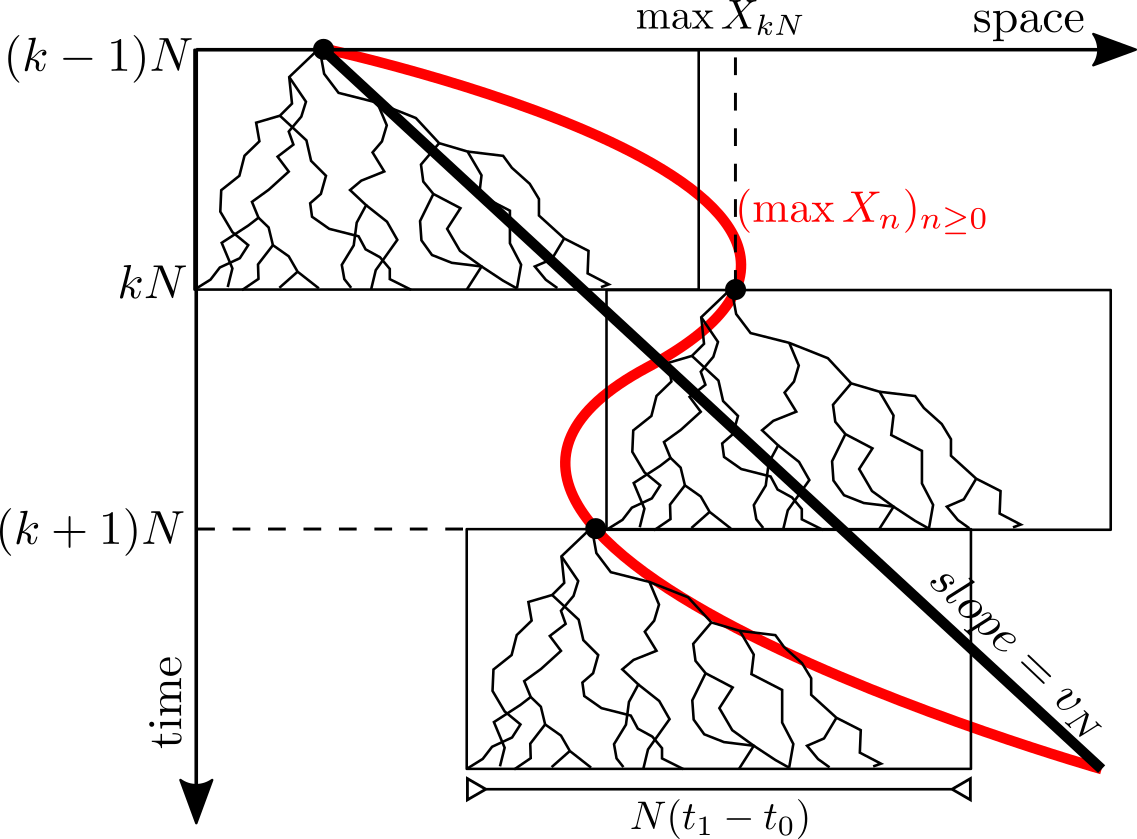
\includegraphics[width=0.45\textwidth]{graphics/g1.png}
% \caption{\label{fig:frog1}This is a figure caption.}
\end{wrapfigure}

If we look at the previous proof, we see that the existence of $v_N$ and $\tilde{v}_N$ (the almost sure and $L^1$ limits of the left- and rightmost particles) when started from $X_0 = N \delta_0$ was shown without relying on Proposition \ref{prop:diameter}. We can in fact deduce Proposition \ref{prop:diameter} by an argument inspired by one of Prof. Berestycki's suggestions:

\begin{proof}[Alternative proof of Proposition \ref{prop:diameter}]
Let $Y = (Y_n)_{n \geq 0}$ be a branching random walk (without selection) with point process $\scr{L}$. Start $Y$ from $\delta_{0}$ noting that initially there is only one particle. It is easy to see that the probability $\rho_1$ that the number of particles in $Y$ has reached $N$ by time $N$ is strictly positive. Define $m_Y$ and $M_Y$ for $Y$ analogously to the definition of $m$ and $M$ in the proof of Proposition \ref{prop:diameter}. By Lemma \ref{lem:ExpTailsMax} one can find $t > 0$ large enough such that $\rho_2 \defeq \PrCond{-t \leq m_Y \leq M_Y \leq t }{\# Y_N \geq N} > 0$. We can now write

\begin{align}\label{eqn:ETBC}
\Pr{\{ \# Y_N \geq N \} \cap \{-t \leq m_Y \leq M_Y \leq t \}} &= \Pr{\# Y_N \geq N} \PrCond{-t \leq m_Y \leq M_Y \leq t }{\# Y_N \geq N} \\
															   &\geq \rho_1 \rho_2 > 0. 
\end{align}
Suppose that we couple $X$ with independent copies of $Y$  placed at the space-time points $(\max X_{kN}, kN)_{k \geq 0}$ denoted by $((Y^{(k)}_n)_{0 \leq n \leq N})_{k \geq 0}$. By the second Borel-Cantelli lemma and (\ref{eqn:ETBC}) it follows that almost surely infinitely many of the $(Y^{(k)}_n)_{0 \leq n \leq N}$ must have $N$ particles by time $N$ and have $-t \leq m_Y \leq M_Y \leq t $. This in turn implies that for infinitely many $k \geq 0$ the diameter is less than $2Nt$ for some time $n \in [Nk, N(k+1))$. This immediately yields $\tilde{v}_N = v_N$. 
\end{proof}

\begin{proposition}[{{\cite[analogue of Proposition 3]{exp_tails}}}]\label{prop:increasing_speed}
The sequence $(v_N)_{N \geq 1}$ is non-decreasing. 
\end{proposition}
\begin{proof}
This is again a consequence of Lemma \ref{lem:monotonicity}. 
\end{proof}

% \begin{remark}\label{rem:constants}
% From Proposition \ref{prop:increasing_speed} we can deduce that $v_N$ increases to a possibly infinite limit $v_\infty$ as $N$ goes to infinity. Assumption \ref{ass:exponential_tails} implies that $\Lambda$ is smooth on the interior of $\cal{D}(\Lambda)$ so that both quantities $v \defeq \psi'(t^*)$ and $\chi \defeq \frac{\pi^2}{2} t^* \psi''(t^*)$ are finite. In Section \ref{sec:ExpTails_BrunDer} we will see that $v_\infty$ is in fact equal to $v$. 
% \end{remark}

\begin{lemma}\label{lem:ExpTailsKingmanHolds}
The random variables $Z_{i,j}$ as defined in the proof of Proposition \ref{prop:ExpTailsSpeedExistence} satisfy the hypothesis of Kingman's Subadditive Theorem. 
\end{lemma}

\begin{proof}
For each $k \geq 1$ the sequence $\{Z_{k, 2k}, Z_{2k, 3k}, ...\} = \{\max X^k_k, \max X^{2k}_k, ... \}$ is i.i.d. so stationary and ergodic. Clearly the distribution of $(Z_{i, i + k})_{k \geq 0} = (\max X^i_k)_{k \geq 0}$ is independent of $i$. $\E Z^+_{0,1} = \E (\max X_1)^+ < \infty$ because $\max X_1 \in L^1$ by (\ref{eqn:ExpTailsMaxIntegrable}). Finally, $\E Z_{0, n} = \E \max X_n \geq n\, \E \scr{L}_{0,1}(1)$. 
\end{proof}











\subsection{Brunet-Derrida behaviour}\label{sec:ExpTails_BrunDer}

We are now ready to present and prove our main result in this section, the analogue of Bérard and Gouéré's Theorem 1:
\begin{theorem}\label{thm:ExpTails_BrunDer}
As $N$ goes to infinity, 
\begin{equation*}
v_N = - \frac{\pi^2 (t^*)^2 \widehat{\psi}''(t^*)}{2 (\log N)^2} + o((\log N)^{-2}). 
\end{equation*}
\end{theorem}

First let us describe the coupling between the $N$-branching random walk and $N$ independent branching random walks which allows us apply Theorems \ref{thm:infty_good} and \ref{thm:finite_good}. Let $(\text{BRW}_j)_{j \in [N]} = ((\bb{T}_j, V_j))_{j \in [N]}$ be $N$ independent copies of the BRW with point process $\scr{L}$. Define $\scr{T}_n \defeq \bigsqcup_{j=1}^N \{ x \in \bb{T}_j \,:\, |x|=n \}$ to be the disjoint union of vertices at depth $n$. We now inductively define a sequence $(G_n)_{n \geq 0}$ of random subsets of $\scr{T}_n$, each with exactly $N$ elements. These random subsets will correspond to the particles alive in the coupled $N$-braching random walk at time $n$. Define $G_0 = \scr{T}_0$ and given $G_n$, define $H_n$ to be the vertices in $\scr{T}_{n+1}$ that descend from vertices in $G_n$. Finally, set $G_{n+1}$ to be the set of $N$ vertices in $H_n$ with the gratest value. If we now define (with some abuse of notation) $\frak{X}_n = \sum_{u,j : u \in G_n \cap \bb{T}_j} \delta_{V_j(u)}$ then $(\frak{X}_n)_{n \geq 0}$ has the same distribution as $X$ started from $N \delta_0$. 
% In what follows we will refer to all of $\bb{T}$, $\Phi$, $\epsilon_{n,i,j}$ and $\tau_{n,i}$ without explicitly explaining the obvious relationships between these objects. Let us now record a technical lemma that will be used in the proof of the lower bound in Theorem \ref{thm:ExpTails_BrunDer}. 

\begin{lemma}[{{\cite[Adapted by Bérard and Gouéré from Lemma 5.2]{pemantle2009search}}}]\label{lem:ExpTailsGoodSequencesTechnical}
Let $v_1 < v_2 \in \R$ and $1 \leq m \leq n \in \N$. Suppose $0 \eqdef x_0, ..., x_n$ is a sequence of real numbers such that $\max_{i \in \bbracket{0, n - 1}} (x_{i+1} - x_i) \leq K$ for some $K > 0$, and define $I \defeq \{ i \in \bbracket{0, n - m} \mid\, x_{i + j} - x_i \geq j v_1,\quad \forall j\in\bbracket{0,m}\}$. If $x_n \geq v_2 n$, then $\#I \geq \frac{v_2 - v_1}{K - v_1}\frac{n}{m} - \frac{K}{K - v_1}$. 
\end{lemma}

\begin{proof}[Proof of upper bound in Theorem \ref{thm:ExpTails_BrunDer}]
As before, we first treat the case $X_0 = N \delta_0$. For notational simplicity define $\sigma^2 = \pi^2 (t^*)^2 \widehat{\psi}''(t^*) / 2$. Our aim is to show $v_N \defeq \lim_{n \to \infty} \Ex{n^{-1} \max X_n} \leq -  \sigma^2 / (\log N)^2 + o((\log N)^{-2})$. Recalling the proof of Proposition \ref{prop:ExpTailsSpeedExistence}, we know by subadditivity that
\begin{equation}\label{eqn:ExpTailsSubaddDecomp1}
v_N \leq \frac{\Ex{\max X_n}}{n} \qquad\qquad\forall\, n \in \N. 
\end{equation}
In light of the desired correction term, we decompose (\ref{eqn:ExpTailsSubaddDecomp1}) into
\begin{equation}
\Ex{\max X_n} = - \frac{\sigma^2}{(\log N)^2} + \Ex{\max X_n \Ind_{\{\max X_n \geq -n \sigma^2 (\log N)^{-2} \}}}. 
\end{equation}
However, this is not the exact form of the RHS that we will work with. Let $\gamma \in (0,1)$ and $\epsilon = \epsilon(N)$ whose precise form we will choose later, but will be approximately $\sigma^2 (\log N)^{-2}$ as $N \to \infty$. We go on to show that in
\begin{equation}
n^{-1} \Ex{\max X_n} =  - (1 - \gamma)\epsilon + n^{-1} \Ex{\max X_n \Ind_{\{\max X_n \geq  -n (1 - \gamma) \epsilon \}}}
\end{equation}
the last term is $o((\log N)^{-2})$. This will yield the desired upper bound on $v_N$ if we take $\gamma \to 0$. We further decompose the problem: for $\delta > 0$ we have
\begin{equation}
n^{-1} \Ex{\max X_n \Ind_{\{\max X_n \geq - n (1 - \gamma)\epsilon \}}} \leq \delta\underbrace{\Pr{\max X_n \geq -n (1 - \gamma)\epsilon }}_{\circled{1}} + \underbrace{\Ex{n^{-1} \max X_n \Ind_{\{ \delta n \leq \max X_n \}}}}_{\circled{2}}. \label{eqn:ExpTailsSubaddDecomp2} 
\end{equation}
First we show that $\circled{1} = o((\log N)^{-2})$, which requires careful scaling the variables involved. Set $n = \ceil{N^\xi}$ for some $0 < \xi < \gamma$ and $m = m(N) \leq n$ whose exact form we'll specify later. Let $B$ be the number of vertices in $\sqcup_{i=0}^n G_i$ that are $(m, - \epsilon)$-good with respect to their corresponding BRWs. Let $u_0, u_1, ..., u_n$ be a path in $\bb{T}_{i_0}$ for some $i_0 \in [N]$ such that $u_0 = root_{i_0}$ and $u_n \in G_n$ with $V_{i_0}(u_n) = \max X_n$. In other words, let $BRW_{i_0}$ be the random walk that the rightmost particle of the coupled $N$-branching random walk lives in at time $n$, and let $u_0, ..., u_n$ be the path connecting it to the root. Define the event $E \defeq \{ \max X_n \geq - n (1 - \gamma)\epsilon \}$, and apply Lemma \ref{lem:ExpTailsGoodSequencesTechnical} to the sequence of real numbers $(V_{i_0}(u_i))_{i \in [n]}$. It follows that on $E$, for any $K > 0$, either one of the random walk steps along the path is $> K$ or $B \geq \frac{\gamma\epsilon}{K + \epsilon}\frac{n}{m} - \frac{K}{K + \epsilon}$. This yields
\begin{equation}\label{eqn:ExpTailsEBound}
\circled{1} = \Pr{E} \leq \Pr{M \geq K} + \Pr{B \geq \frac{\gamma\epsilon}{K + \epsilon}\frac{n}{m} - \frac{K}{K + \epsilon}},  
\end{equation}
where $M \defeq \max \{\max \scr{L}_{l, j} \mid\, l \in \bbracket{0, n - 1},\, j \in [N]\}$. Set $\beta \in (0, \bb{V}(X))$ and let $\theta > 0$ be as in Theorem \ref{thm:finite_good}. Let $\lambda > 0$, and define 
\begin{equation}
m \defeq \ceil*{ \left[\frac{2 \theta}{\pi^2}\right]^{3/2} \left( \frac{(1 + \lambda) \log N}{(\bb{V}(X) - \beta)^{1/2}}\right)^3},
\end{equation} 
and $\epsilon \defeq \theta\, m^{-2/3}$. $m$ is carefully chosen so that by Theorem \ref{thm:finite_good}, 
\begin{equation}\label{eqn:ExpTailsProof}
\rho(m, \epsilon) \leq N^{-(1 + \lambda)} 
\end{equation}
for all large $N$. Also let $K = \kappa \log N$ for $\kappa > 0$ and observe that $\frac{\gamma\epsilon}{K + \epsilon}\frac{n}{m} - \frac{K}{K + \epsilon} > 0$ for large enough $N$ independently of $\kappa$. Thus (\ref{eqn:ExpTailsEBound}) turns into
\begin{equation}
\circled{1} = \Pr{E} \leq \underbrace{\Pr{M \geq K}}_{\circled{1a}} + \underbrace{\Pr{B \geq 1}}_{\circled{1b}}. 
\end{equation}

$\circled{1a}$: As noted before, $(\max \scr{L}_{i,j})_{i \geq 0, j \in [N]} = (\scr{L}_{i, j}(1))_{i \geq 0, j \in [N]}$ are i.i.d. with common distribution $\max \scr{L}$ and have exponentially decaying tails so that there exists $C, \phi, K_0 > 0$ such that for all $K > K_0$ it holds that $\Pr{\max \scr{L} > K} \leq C \exp(-\phi K)$. By a calculation similar to the proof of Lemma \ref{lem:ExpTailsMax}, for all large enough $\kappa$ we get
\begin{align}
\Pr{M \geq K} &= 1 - (1 - \Pr{\max \scr{L} > K})^{Nn} \leq 1 - (1 - C \exp(-\phi K))^{Nn} \\
			  &= 1 - (1 - C N^{-\phi \kappa})^{Nn} \leq C N^{-\phi \kappa} Nn = C N^{1 + \xi - \phi \kappa}. 	
\end{align} 
Thus, $\Pr{M \geq K} = o((\log N)^{-2})$ for $\kappa > 2/\phi$. \\

$\circled{1b}$: Consider a vertex $u \in \bb{T}_{j_0}$ for some $j_0 \in [N]$ with $|u| \leq n$. The event $\{u \in G_d\}$ is measurable with respect to the sigma algebra generated by the random variables $\{ V_j(v) \mid\, j \in [N],\, v \in \bb{T}_j,\, |v| \leq |u|\}$. On the other hand, the event $\{ u \text{ is }(m, - \epsilon) \text{-good}\}$ is determined by the variables $\{ V_{j_0}(v) - V_{j_0}(u) \mid\, v \in \bb{T}_{j_0},\, |u| < |v| \}$, so that the two events are independent. We can write $B$ as 
\begin{equation*}
B = \sum\limits_{i=1}^N \sum\limits_{u \in \bb{T}_i} \Ind_{\{u \text{ is } (m, - \epsilon)\text{-good}\}} \Ind_{\{u \in G_d \text{ for some d} \leq n \}}. 
\end{equation*}
Taking expectations gives 
\begin{equation}
\Ex{B} \leq N(n+1)\rho(m, \epsilon) = \cal{O}(N^{\xi -\lambda}) = o((\log N)^{-2}) \qquad\text{as $N$ goes to infinity}, 
\end{equation}
where we used that $G_n$ has $N$ elements for all $n$. Applying Markov's inequality to $B$ and combining with our estimate of $\circled{1a}$ gives $\circled{1} = o((\log N)^{-2})$ as desired. \\

We now turn to showing $\circled{2} = o((\log N)^{-2})$. Consider the obvious inequality $\exp(\max X_n) \leq \sum_{j \in [N]} \sum_{x \in \bb{T}_j : |x| = n} \exp(V_j(x))$. It follows from the Many-to-One lemma that 
\begin{align}
\Ex{\exp(\max X_n)} \leq N\, \E\sum\limits_{|x| = n} \exp(V(x)) = N. 
\end{align}
Now apply Lemma \ref{lem:ExpTailBound} with $x = \max X_n$ and $a = \delta n$ and take expectations to get 
\begin{align*}
\Ex{\max X_n \Ind_{\{\max X_n \geq \delta n \}}} &\leq \Ex{\exp(X_n - \delta n / 2)} \leq N \, e^{-\delta n / 2} = o((\log N)^{-2}).
\end{align*}
This concludes the proof of the upper bound: we have shown that for any choice of $\gamma \in (0,1)$, $\beta \in (0, \bb{V}(X))$ and $\lambda > \xi > 0$ we have
\begin{equation}\label{eqn:ExpTailResultTally}
v_N \leq \Ex{\ceil{N^\xi}^{-1} \max X_{\ceil{N^\xi}}} \leq - (1 - \gamma) \frac{\pi^2 (\bb{V}(X) - \beta)}{2 (1 + \lambda)^2(\log N)^2} + o((\log N)^{-2}). 
\end{equation}
Taking $\gamma, \beta, \lambda$ and $\xi$ to zero gives the desired result. 
\end{proof}











\begin{proof}[Proof of lower bound in Theorem \ref{thm:ExpTails_BrunDer}]

Let $\lambda, \eta \in (0,1)$ and let $\epsilon \defeq \pi^2 \bb{V}(X) 2^{-1} (1-\lambda)^{-2}(\log N)^{-2}$. With this choice Theorem \ref{thm:infty_good} gives $\rho(\infty, - \epsilon) = N^{\lambda - 1 + o(1)}$ as $N \to \infty$. Recall now the construction of $(X^l_n)_{n, l \geq 0}$ using $(\scr{L}_{n, j})_{n \geq 0, j \in [N]}$ from the proof of Proposition \ref{prop:ExpTailsSpeedExistence}. Define the random variables $\Gamma_0 \defeq 0$ and $J_0 \defeq 0$ and set $i = 0$. Given $\Gamma_i$ and $J_i$ inductively define $L_{i+1} \defeq n \land \inf\{ k \mid\, \min X^{\Gamma_i}_k \geq -(1+\eta)\epsilon k\}$. Finally, let $\Gamma_{i+1} \defeq \Gamma_i + L_{i+1}$ and $J_{i+1} \defeq J_i + \min X^{\Gamma_i}_{L_{i+1}}$. By Lemma \ref{lem:monotonicity} it follows that 
\begin{equation}\label{eqn:regenTime}
\min X_{\Gamma_i} \geq J_i \qquad\forall\, i \geq 0. 
\end{equation}
Observe now that $\Gamma_{i+1} - \Gamma_i$ is an i.i.d. sequence with common distribution $L \defeq n \land \inf \{ k \mid \min X_k \geq - (1+\eta)\epsilon k\}$. Similarly, the sequence $J_{i+1} - J_i$ is also i.i.d. with common distribution $\min X_L$. The strong law of large numbers gives 
\begin{equation}
\lim\limits_{i \to \infty} \frac{\min X_{\Gamma_i}}{i} = \lim\limits_{i \to \infty} \frac{\min X_{\Gamma_i}}{\Gamma_i} \frac{\Gamma_i}{i} = v_N \E L
\end{equation}
almost surely. However, by (\ref{eqn:regenTime}) we also have
\begin{equation}
\liminf\limits_{i \to \infty} \frac{\min X_{\Gamma_i}}{i} \geq \liminf\limits_{i \to \infty} \frac{J_i}{i} = \Ex{\min X_L}.
\end{equation}
Denote $B \defeq \{ \min X_k < - (1+\eta)\epsilon \text{ for all } k \in [n]\}$ and define the random variable $\Theta_n$ to have the law of $\min \{\min \scr{L}_{i, j} \mid\, j \in [N],\, 0 \leq i \leq n - 1 \}$. Combining the obvious inequalities $\min X_L \geq -(1 + \eta)\epsilon L \Ind_{\{B^c\}} + n \Theta_n \Ind_B$ and $1 \leq L \leq n$ with the above bounds we get
\begin{equation}\label{eqn:lowerBdd}
v_N \geq \frac{\Ex{\min X_L}}{\E L} \geq -(1+\eta)\epsilon (1 + n\Pr{B}) - n\Ex{|\Theta_n| \Ind_B}. 
\end{equation}
By Hölder's inequality $\Ex{|\Theta_n| \Ind_B} \leq \sqrt{\Ex{\Theta_n^2}\Pr{B}}$. By Lemma \ref{lem:ExpTailsMax} we know that $\Theta_n$ has exponentially decaying tails, so in particular is square-integrable. To prove the lower bound we only need a suitably strong upper bound on $\Pr{B}$. The remainder of the proof is dedicated to this. \\

Since $1 < \Ex{\#\scr{L}} = \E\sum_{|x|=1} \Ind$, by the monotone convergence theorem we can take $R \in \R$ such that $1 < \E\sum_{|x|=1} \Ind_{\{ V(x) \geq R\}}$. If we let $(M_n)_{n \geq 0}$ be the Galton Watson process started from $1$ with offspring law $\sum_{|x|=1} \Ind_{\{ V(x) \geq -R\}}$ then by Lemma \ref{lem:ExpTailsGW} there exist $\phi > 1$ and $r > 0$ such that $\Pr{M_n \geq \phi^n} \geq r$ for all $n \geq 0$. Define now $s \defeq \ceil{\frac{\log N}{\log \phi}} + 1$ and $m \defeq \ceil{\frac{- Rs}{\eta\, \epsilon}}$ and finally set $n = s + m$. Consider a vertex $u$ at depth $m$ in one of the $BRW_i$. The probability that there are at least $\phi^s$ distinct paths $u \eqdef u_m, ..., u_n$ with $V_i(u_{k+1}) - V_i(u_k) \geq R$ for all $k \in \bbracket{m, n - 1}$ is greater than $r$ by our previous discussion. Recall that the probability of the root being $(m, - \epsilon)$-good is $\rho(m, - \epsilon)$. We see that then the probability of observing a path $root = w_0, ..., w_n$ in $BRW_i$ such that $V_i(w_k) \geq - k \epsilon$ for $k \in [m]$ and $V_i(w_{k+1}) - V_i(w_k) \geq R$ for $k \in \bbracket{m, n-1}$ is at least $\rho(m, - \epsilon) r$. By the choice of $s$ and $m$, such a path must also be $(n,  - (1+\eta)\epsilon)$-good. For $i \in [N]$ define $A_j$ to be the event that $BRW_i$ contains no more than $\phi^s$ distinct $(n, - (1+\eta)\epsilon)$-good paths starting at the root. By independence we get
\begin{equation}
\Pr{\bigcap\limits_{i=1}^N A_i} \leq (1 - \rho(m, \epsilon) r)^N. 
\end{equation}
On the event $B \cap [\cap_{i=1}^N A_i]^c$ one of the $BRW_i$s has $> \phi^s > N$ particles at time $n$ that have stayed to the right of the space time line with slope $ - (1 + \eta)\epsilon$ until time $n$. By definition, on $B$ this implies that there are $> N$ particles alive in the $N$-branching random walk which is impossible. Therefore we must have $B \subset \cap_{i=1}^N A_i$. Using the fact that $\rho(m, - \epsilon) \leq \rho(\infty, - \epsilon) = N^{\lambda - 1 + o(1)}$ and the inequality $1 - x \leq \exp(-x)$ for all $x \in \R$, we get
\begin{equation}\label{eqn:ExpTailsBBound}
\Pr{B} \leq \Pr{\bigcap\limits_{i=1}^N A_i} \leq \exp(-N^{\lambda + o(1)})
\end{equation}
Combining the above estimate of $\Pr{B}$ with (\ref{eqn:lowerBdd}) results in 
\begin{equation}
v_N \geq - \frac{\pi^2 (1 + \eta) \bb{V}(X)}{2 (1 - \lambda)^2(\log N)^2} + o((\log N)^{-2}). 
\end{equation} 
As $\lambda$ and $\eta$ can be taken arbitrarily small, the desired result follows. 
\end{proof}

\subsection{Discussion}
This section is based in part on \cite{exp_tails} Section 8. Write $v_N$ for the asymptotic speed of the $N$-BRW and $v \defeq \lim_{N \to \infty} v$ for its limit, to which it converges at rate $(\log N)^{-2}$. The proof of the Brunet-Deridda behaviour hinged on the idea that the following two are comparable:
\begin{enumerate}[(a)]
\item \vspace{-1mm} $(BRW_j)_{j \in [N]}$ do not survive killing below the speed $v - \epsilon$
\item \vspace{-3mm} $v_N < v - \epsilon$. 
\end{enumerate}
\vspace{-3mm}
It is intuitively clear why this might be true: if $(a)$ holds then we certainly can't expect the $N$-BRW to propagate faster than $v - \epsilon$ since it is dominated by $(BRW_j)_{j \in [N]}$ through the coupling introduced in section \ref{sec:ExpTails_BrunDer}. Conversely, suppose $(a)$ doesn't hold. Consider the particle in the $N$-BRW at time zero that corresponds to a $BRW_i$ that survives killing. With probability $ \sim 1/N$ the descendants of this particle will survive and form the entirety of the $N$-BRW. If this doesn't happen we can `restart' the argument. After a rougly geometric number of attempts we will succed in which case $(b)$ cannot hold. \\

To make such an argument rigorous we needed to get a handle on the probability of a $BRW$ exhibiting paths of various slopes and lengths near the critical slope $0$; the expectation of the $BRW$'s associated random walk. In \cite{gantert2008asymptotics} they did just that using the Many-to-One lemma and one of Mogulskii's results which accurately describes the probabilitiy of a centred random walk's path to stay in a general space-time region. Loosely speaking they show that on the scale $m \propto \epsilon^{-u}$ for $u \in (0, 3/2]$ we have
\begin{equation}
\log \rho(m, -\epsilon) \propto - \epsilon^{-u/3}\qquad\text{as } \epsilon \downarrow 0. 
\end{equation}
Similarly, they show $\log\rho(\infty, -\epsilon) \propto - \epsilon^{1/2}$ as $\epsilon \downarrow 0$. Using this the convergence rate $(\log N)^{-2}$ can be heuristically deduced: setting $\epsilon_N = v - v_N$ we would expect 
\begin{equation}\label{eqn:speed_scale_heuristic}
\rho(\infty, - \epsilon_N) \propto \frac{1}{N}. 
\end{equation}
To see why, suppose for contradiction that $\rho(\infty, - \epsilon_N) \ll 1_N$. Then with probability close to one none of the $BRW_i$ survive killing which would imply that $v_N$ needs to be slower. Conversely, if we had $\rho(\infty, - \epsilon_N) \gg 1/N$ then with probability close to one at least one of the $BRW_i$ would survive killing, implying that $v_N$ needs to be faster. From \ref{eqn:speed_scale_heuristic} and the asymptotic form of $\rho(\infty, -\epsilon)$ for small $\epsilon$ it follows that for all large $N$, $\epsilon_N$ should satisfy
\begin{equation}
\epsilon_N \propto (\log N)^{-2}. 
\end{equation}